% 负责人：B / onlysonder，对应 #3、#4。
\section{已知结构分类与解释}

\subsection{输入、模型与训练}
分类输入是 WT 两个重复中的 688 个窗口，对应 344 个已知结构位置；每个窗口是
$128\times128$ 的 float32 接触矩阵，标签顺序为 OPCID、CHIN、CHID。沿用共享预处理
给出的固定分组，train/val/test 分别为 482、102、104 个窗口。测试集有 OPCID 20、
CHIN 76、CHID 8 个窗口，即 52 个位置、每个位置两个重复。按结构窗口重叠连通分量
分组后，三个集合间没有共享窗口位置。

分类器为三层小型 CNN，卷积通道数为 16、32、64，每层后接批归一化、ReLU 和
$2\times2$ 最大池化，再用全局平均池化和线性层输出三类分数，共 23,603 个参数。
训练使用训练集类别权重、加权交叉熵与 Adam（学习率 $10^{-3}$、权重衰减 $10^{-4}$、
dropout=0.3），随机种子为 20260918，batch size 为 32，最多训练 30 轮，patience 为 8；
只依据验证集 Macro-F1 选取权重。

组长 9 月 22 日的正式训练记录对应另一份 checkpoint：最佳轮次 13，验证集 Accuracy
0.6961、Macro-F1 0.5861。输入交接包没有包含该权重。为完成固定测试评价，B 在 CPU 上
按相同数据、划分、种子和超参数单独复跑，得到新 checkpoint（SHA-256 见
\url{docs/results/classifier/test_evaluation/verification.json}）。这次运行 20 轮后早停，
最佳轮次为 12，验证集 Accuracy=0.6667、Macro-F1=0.5674。以下测试结果全部对应 B 的
新 checkpoint，不与组长原 checkpoint 的验证指标混写；训练和分析命令、输入及代码
指纹保存在 \url{docs/results/classifier/test_evaluation/}。

\subsection{固定测试集与基线}
固定训练完成后，使用配套的 \texttt{splits.csv} 对 104 个测试窗口进行一次最终评价，
未按随机种子重新划分，也未依据测试结果调整模型。CNN 的测试 Accuracy 为 0.5096，
Macro-F1 为 0.3454。逐类结果如下：

\begin{center}
\small
\begin{tabular}{lrrrr}
\toprule
类别 & 支持数 & Precision & Recall & F1 \\
\midrule
OPCID & 20 & 0.2955 & 0.6500 & 0.4062 \\
CHIN & 76 & 0.7843 & 0.5263 & 0.6299 \\
CHID & 8 & 0.0000 & 0.0000 & 0.0000 \\
\bottomrule
\end{tabular}
\end{center}

混淆矩阵的行是真实类别、列是预测类别，顺序为 OPCID、CHIN、CHID；数值和图片
分别保存在 \url{docs/results/classifier/test_evaluation/confusion_matrix_test.csv} 与
\url{docs/results/classifier/test_evaluation/confusion_matrix_test.png}。

\begin{center}
\small
\begin{tabular}{lrrr}
\toprule
真实 / 预测 & OPCID & CHIN & CHID \\
\midrule
OPCID & 13 & 7 & 0 \\
CHIN & 27 & 40 & 9 \\
CHID & 4 & 4 & 0 \\
\bottomrule
\end{tabular}
\end{center}

我们比较两个只在训练集上拟合的基线：始终预测训练多数类 CHIN，以及将 $128\times128$
矩阵展平后拟合、带 balanced 类权重的逻辑回归。逻辑回归参数为
\texttt{max\_iter=1000}、\texttt{solver=lbfgs}、\texttt{random\_state=20260918}，
训练过程没有收敛警告。

\begin{center}
\small
\begin{tabular}{lrrrrrr}
\toprule
方法 & $n$ & Accuracy & Macro-F1 & OPCID F1 & CHIN F1 & CHID F1 \\
\midrule
小型 CNN & 104 & 0.5096 & 0.3454 & 0.4062 & 0.6299 & 0.0000 \\
多数类（CHIN） & 104 & 0.7308 & 0.2815 & 0.0000 & 0.8444 & 0.0000 \\
逻辑回归 & 104 & 0.8365 & 0.5644 & 0.8000 & 0.8931 & 0.0000 \\
\bottomrule
\end{tabular}
\end{center}

CNN 的 Macro-F1 高于多数类基线，但 Accuracy 更低；逻辑回归在这次固定测试划分上的
Accuracy 和 Macro-F1 都高于 CNN。CNN 将 51 个窗口预测为 CHIN、44 个预测为 OPCID、
9 个预测为 CHID；它没有退化成始终输出多数类，但把 27 个真实 CHIN 判成 OPCID。
三个方法都没有正确识别 CHID，测试集中该类仅有 8 个窗口（4 个独立位置），这是当前
最明显的局限。结果只反映这一固定划分，不据此声称 CNN 优于简单方法。

测试失败案例文件保存在 \url{docs/results/classifier/test_evaluation/failure_cases.csv}。
例如，真实 \texttt{CHIN\_218} 被以 0.8853 的分数判为 OPCID；真实 \texttt{OPCID\_12} 被判为 CHIN；
真实 \texttt{CHID\_8} 被判为 CHIN（CHIN/CHID 分数分别为 0.5431/0.4312）。这些案例表明模型
仍会混淆不同结构类别，尤其难以区分少数类 CHID；不能只凭显著性图将这些响应解释成
生物学机制。

\subsection{Grad-CAM 解释}
每类选取了 3 个不同结构位置，图中并列显示原始分类输入与针对模型预测类别的末层卷积
Grad-CAM 叠加。图像、全部 9 个样本的 ID 和真实/预测标签见
\url{docs/results/classifier/test_evaluation/gradcam/} 与
\url{docs/results/classifier/test_evaluation/gradcam_examples.csv}。以下各展示一个例子；
CHID 例子预测错误，因此 CAM 针对模型预测的 CHIN 类，而不是将其标成正确识别。
Grad-CAM 表示模型对给定预测类别的相对空间响应，不是因果解释，也不能单独证明
接触结构的生物学机制。

\begin{figure}[htbp]
\centering
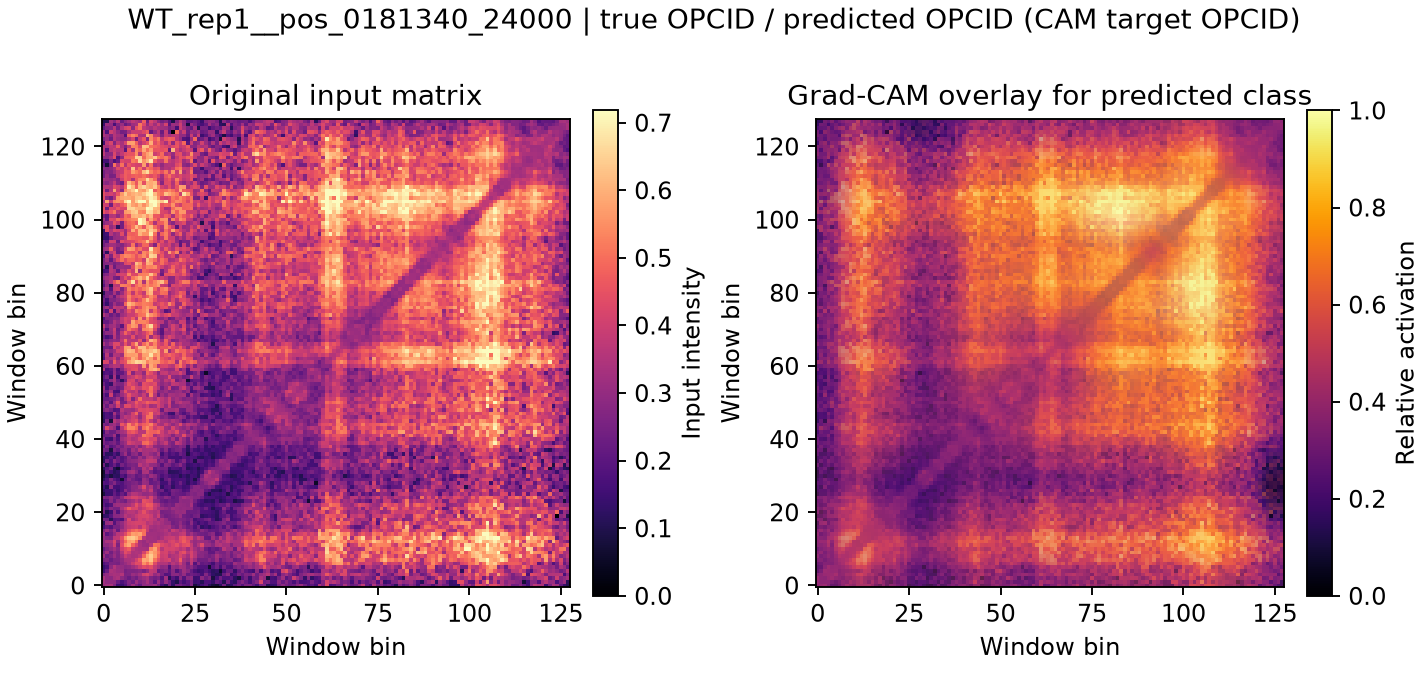
\includegraphics[width=0.72\linewidth]{../results/classifier/test_evaluation/gradcam/WT_rep1__pos_0181340_24000.png}\\[0.35em]
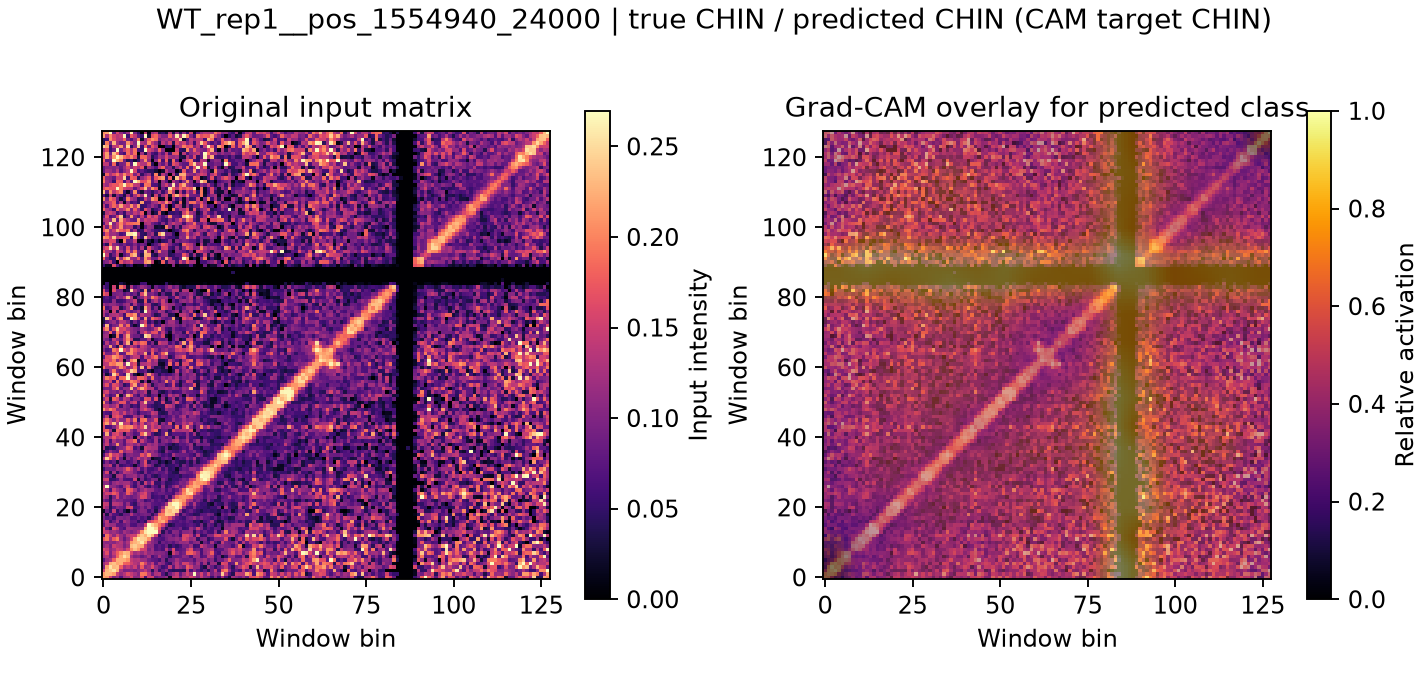
\includegraphics[width=0.72\linewidth]{../results/classifier/test_evaluation/gradcam/WT_rep1__pos_1554940_24000.png}\\[0.35em]
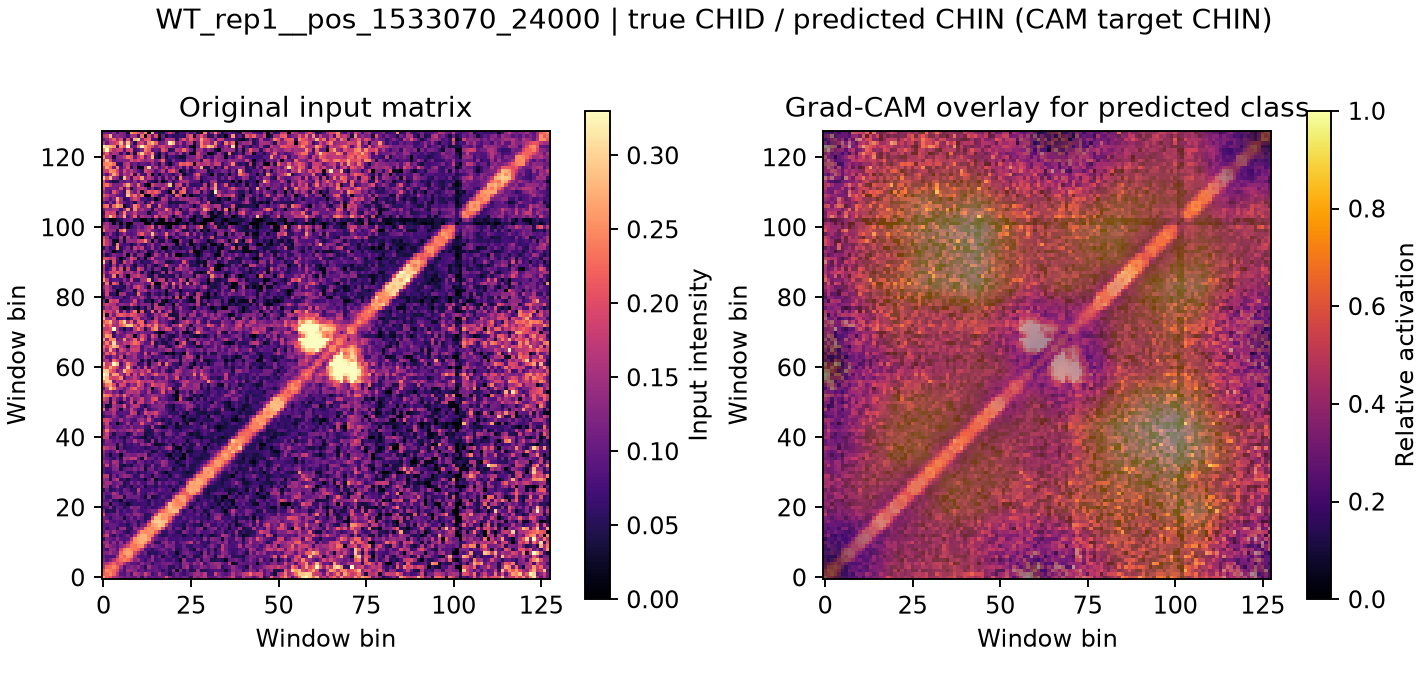
\includegraphics[width=0.72\linewidth]{../results/classifier/test_evaluation/gradcam/WT_rep1__pos_1533070_24000.png}
\caption{测试集代表性 Grad-CAM：依次为 OPCID（预测正确）、CHIN（预测正确）和 CHID（真实类别 CHID，被预测为 CHIN）。每个样本左侧为原输入矩阵，右侧为针对预测类别的相对显著性叠加。}
\label{fig:classifier-gradcam}
\end{figure}
